\section{Background}

\subsection{General architecture of document management systems}

A document management system is a typical client-server model: a document
management server stores the documents (and possibly images, other associated
files) in a document repository, which can be accessed via various interfaces.
The other part of the system is a client, which has built-in support for
opening, saving and editing documents:

\begin{figure}[H]
\centering
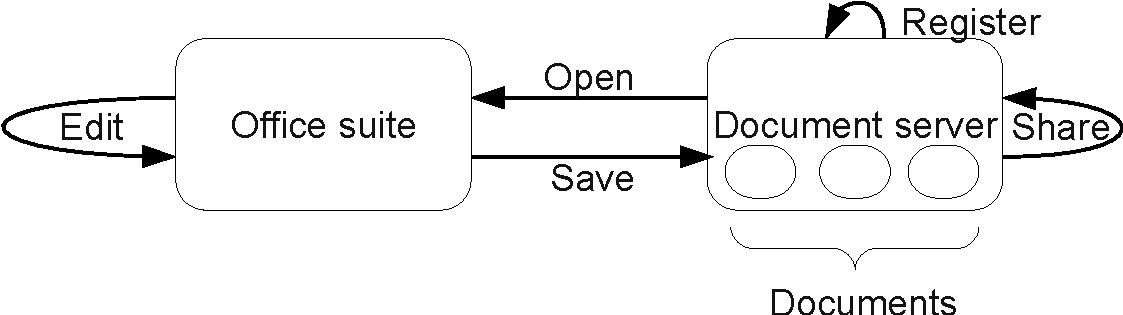
\includegraphics[width=300px,keepaspectratio]{general-arch-of-doc-mgmt-systems.pdf}
\caption{Architecture of a document management system}
\end{figure}

The document management server has registered users. Properties to users (full
name, email, password) are stored on the server.

Every user has document workspaces. Workspaces can have documents, links and
tasks. A workspace can be shared with different permissions (read-only,
read-write), and that is typically done by sending an invitation email which
the other user can accept.

A user may access the document server using a web browser, or via fat client
applications. The advantage of the web browser interface is that it can be
accessed from almost everywhere, however document editing can't be performed.
If such operation should be performed, then the user has to manually download
the document, edit then upload it. This method occasionally does not cause a
problem, but of course it's uncomfortable for daily work.

The other interface is a fat client, which is installed on the machine of the
user. Vendors like to produce a corresponding client for their server,
Microsoft Sharepoint and Microsoft Office is a typical setup.

It is important to note that of course a single server may serve multiple
clients. Also, the same client may connect to multiple servers, however in
practice a central server provides a document storage for all the collaborating
users.

In case of servers or clients speaking different communication protocols,
selection of the used protocol is selected differently on client and server
side. Servers can listen on different addresses, and in this case the address
identifies not only the server, but the used protocol as well.

For example Alfresco\cite{alfresco}, which is an open-source alternative to
Sharepoint, has its native protocol, but also (more or less) can speak the
Sharepoint protocol. As a result, it can be configured to listen on
\emph{http://project:8080/} as an Alfresco server, and on
\emph{http://localhost:7070} as a Sharepoint server.

Clients can have different extensions or plug-ins to handle different
protocols. For example Microsoft Office can accept Sharepoint URL-s in the
standard file opener dialog, while the Alfresco extension for OpenOffice.org
has a dedicated menu in the application to connect to an Alfresco server.

It is also common that the client extensions have minimal business logic. For
example the proprietary Sharepoint extension to OpenOffice.org, created by
Oracle can't talk to every Sharepoint server, like Microsoft Office does -- as
long as a server-side component provided by Oracle is not installed on the
server. While this approach may be compelling during development, actually it
is uncomfortable for system administrators.

As a result, I paid attention in my solution to not require such additional
server-side component installation.

\subsection{Related standards}

The specification called Content Management Interoperability
Services\cite{cmis} is created to address compatibility issues between various
document management server implementations. OASIS approved it on May 1, 2010,
so it's relatively new. Also, at the time of writing implementation is far from
complete among major document management servers. Alfresco 3.3 implements the
client side only, Sharepoint 2007 does not support it yet, so at the moment
it's a vision that all major document servers will implement this
specification.

On the other hand, there are a lot of implementations in other products, such
as IBM Lotus Connections 3.0\cite{lotus} (server side only) or TYPO3 (client
and server side).

CMIS has two main goals:

\begin{itemize}
\item Providing a list of web service (SOAP) interfaces, it's language-independent.
\item It allows separating the service and content, making it possible to
implement services for legacy document repositories without modifying them.
\end{itemize}

To achieve this, it defines a domain model, describing the following data model
elements:

\begin{itemize}
\item repository: a container
\item object: common ancestor for document, folder, relationship and policy objects
\item object-type: a set of properties, all instances of a type have those
\item document object: the document entities managed by the repository
\item folder object: container for file objects
\item relationship object: representing links between objects
\item policy object: policies enforced by a repository
\item access control: consists of pre-defined permissions and allows defining new ones
\item versioning: versions document objects (other object types are not allowed)
\item query: type-based query to list objects matching a specified criteria
\item change log: changes to objects since a given timestamp
\end{itemize}

Then -- using this data model -- it specifies services to operate on them:

\begin{itemize}
\item common service elements: includes paging, exception handling
\item repository services
\item navigation services
\item object services: includes factory functions for different object types
\item multi-filing services: makes it possible to add/remove objects to folders
\item discovering services: to search query-able objects within a repository
\item versioning services: includes check in, check out, cancel checkout, get
	versions
\item relationship services: provides the relationships of an object
\item policy services: apply and remove policies, list applied ones
\item ACL services: get and apply an ACL
\end{itemize}

Finally it explains concrete syntaxes: the Restful AtomPub Binding and the Web
Services (SOAP) binding.
